\documentclass[aspectratio=169,11pt]{beamer}
\usepackage[dvipsnames]{xcolor}
\usepackage{tikz}
\usepackage{mathtools}
% \usepackage{lmodern}      % replaces Computer Modern with Latin Modern
% \usepackage{inconsolata}
\usepackage{multirow}
\usepackage[style=authoryear-comp,url=false,date=year,doi=false,isbn=false,eprint=true,maxnames=1,minnames=1,backend=biber,natbib=true]{biblatex}
% ------------------------------------------------------------
% MIT COLOR PALETTE  (from MIT Brand Guidelines)
% ------------------------------------------------------------
\definecolor{mitred}{HTML}{A31F34}       % Primary MIT rednn
\definecolor{mitdarkgray}{HTML}{545454}  % Neutral dark gray
\definecolor{mitlightgray}{HTML}{C7C7C7} % Light gray
\definecolor{mitorange}{HTML}{D56F00}    % Secondary accent
\definecolor{mitblue}{HTML}{8A8BFF}      % Accent cool tone

% ------------------------------------------------------------
% APPLY TO TITLES
% ------------------------------------------------------------
% Title of the entire talk (front page)
\setbeamercolor{title}{fg=mitred}
\setbeamercolor{subtitle}{fg=mitdarkgray}

% Frame title (top of each slide)
\setbeamercolor{frametitle}{fg=mitred}
\setbeamercolor{framesubtitle}{fg=mitdarkgray}

% Optional: section headings / TOC colors
\setbeamercolor{section title}{fg=mitred}
\setbeamercolor{subsection title}{fg=mitdarkgray}

% --- Bullets / enumeration (structure color drives itemize/enumerate) ---
\setbeamercolor{structure}{fg=mitred}              % bullets, numbers, mini-frames
\setbeamercolor{itemize item}{fg=mitred}
\setbeamercolor{itemize subitem}{fg=mitdarkgray}
\setbeamercolor{enumerate item}{fg=mitred}
\setbeamercolor{enumerate subitem}{fg=mitdarkgray}

% --- Captions (Figure/Table labels & text) ---
\setbeamercolor{caption name}{fg=mitred}           % “Figure”, “Table”
\setbeamercolor{caption}{fg=mitdarkgray}           % caption body text
% Optional: show numbers on captions
% \setbeamertemplate{caption}[numbered]

% --- Blocks ---
\setbeamertemplate{blocks}[rounded][shadow=false]  % or shadow=true for dropshadow
% Normal block: neutral title, neutral body
\setbeamercolor{block title}{fg=mitred,bg=mitorange!20}
\setbeamercolor{block body}{fg=mitdarkgray,bg=mitorange!20}
% Alert block: MIT red title; body neutral
\setbeamercolor{block title alerted}{fg=mitred,bg=mitred!20}
\setbeamercolor{block body alerted}{fg=mitdarkgray,bg=mitred!20}
% Example block: cool accent for contrast
\setbeamercolor{block title example}{fg=mitred,bg=mitdarkgray!20}
\setbeamercolor{block body example}{fg=mitdarkgray,bg=mitdarkgray!20}

% --- Emphasis & inline alerts ---
\setbeamercolor{alerted text}{fg=mitred}           % \alert{...}
\setbeamercolor{example text}{fg=mitblue}

% --- Navigation symbols / progress bars (if your theme uses palettes) ---
\setbeamercolor{palette primary}{fg=white,bg=mitred}
\setbeamercolor{palette secondary}{fg=white,bg=mitdarkgray}
\setbeamercolor{palette tertiary}{fg=white,bg=mitdarkgray}
\setbeamercolor{palette quaternary}{fg=white,bg=mitdarkgray}

% --- Rules, separators, fine lines (optional) ---
\setbeamercolor{separation line}{bg=mitlightgray}
\setbeamercolor{fine separation line}{bg=mitlightgray}

% --- Links ---
\hypersetup{
  colorlinks=true,
  linkcolor=mitred,        % TOC/internal links
  urlcolor=mitred,         % URLs
  citecolor=mitdarkgray    % citations (neutral)
}

\setbeamersize{text margin left=0.5cm, text margin right=0.5cm}


% \setbeamertemplate{footline}[frame number]
\setbeamertemplate{navigation symbols}{}

\setbeamertemplate{footline}{%
  \leavevmode%
  \usebeamerfont{footline}
  \usebeamercolor[fg]{footline}
  \tiny
  \tikz[remember picture, overlay,xscale=0.875,transform shape]{
    \node[anchor=south] at (current page.south) {\insertshorttitle};
    \node[anchor=south west] at (current page.south west) {Sungho Shin--- \href{mailto:sushin@mit.edu}{\tt sushin@mit.edu}};
    \node[anchor=south east] at (current page.south east) {\insertframenumber/\inserttotalframenumber};
  }  
}



% \setbeamertemplate{footline}{%
%   \leavevmode%
%   \hbox to \paperwidth{%
%     \tiny
%     \hspace{.3ex}
%     Sungho Shin---\url{sushin@mit.edu}%
%     \hfil%
%     \insertshorttitle%
%     \hfil%
%     \insertframenumber{}/\inserttotalframenumber
%     \hspace{.3ex}%
%   }%
%   \vspace*{.3ex}%
% }

\setbeamercolor{footline}{fg=mitdarkgray} % or mitred if you like the accent
\setbeamerfont{footline}{size=\scriptsize} % adjust if too big



% \DeclareDelimFormat[bib]{nametitledelim}{\newline\bibsentence}
\addbibresource{shin.bib}
\AtEveryCitekey{\clearfield{pages}} 
\AtEveryCitekey{\clearfield{volume}}
\AtEveryCitekey{\clearfield{number}}
\AtEveryCitekey{\clearfield{primaryclass}}
\AtEveryCitekey{\clearfield{edition}}
\AtEveryCitekey{\clearfield{publisher}}
\AtEveryCitekey{\clearfield{series}}
\AtEveryCitekey{\clearfield{address}}
\DeclareNameAlias{default}{labelname}
\renewbibmacro{in:}{}


% % Only print family name(s), but allow et al. when truncated
% \DeclareNameFormat{author}{%
%   \ifthenelse{\value{listcount}=1}
%     {\namepartfamily} % print first name as last name
%     {\ifnumgreater{\value{listcount}}{\value{liststop}}
%         {\addspace et al.} % print "et al." when beyond maxnames
%         {\namepartfamily}} % otherwise print the next last name
% }
% \DeclareNameAlias{default}{last} % = Lastname, F.


\newcommand{\refbr}[2][]{%
  \begin{tikzpicture}[remember picture, overlay,xscale=0.875,transform shape,inner sep=2pt]
    \node[anchor=south west,align=left,font=\tiny,color=mitdarkgray,text width=1.2\linewidth,yshift=10pt] at (current page.south west) {#1 #2};
  \end{tikzpicture}%
}

\newcommand{\joint}[2][]{% 
  \begin{tikzpicture}[remember picture, overlay, xscale=0.875,transform shape,inner sep=2pt]
    \node[anchor=south west,align=left,font=\tiny,color=mitdarkgray] at (current page.south west) {#1 #2};
    \node[anchor=south east,align=left,font=\tiny,color=mitdarkgray] at (current page.south east) {\insertframenumber/\inserttotalframenumber};  
  \end{tikzpicture}%
}

\graphicspath{{figs/}}

\title[NLP on GPUs: Pivoting-Free IPM]{Solving Large-Scale, Sparse, Constrained Nonlinear Optimization Problems on GPUs}
\subtitle{Pivoting-Free Interior-Point Methods}
\author{
  Sungho Shin\\
  \url{shin.mit.edu}
}
\institute{
  Massachusetts Institute of Technology
}

\date{2025 INFORMS Annual Meeting \\ October 27, 2025}

\begin{document}

\frame{
  \joint{
    Joint work with:
    Alexis Montoison (Argonne),
    François Pacaud (MINES-Paris),
    Mihai Anitescu (Argonne)
  }
  \thispagestyle{empty}
  \titlepage
} % Title page

\setbeamertemplate{footline}[content]
\begin{frame}{Who are we?}
  \begin{center}
    \url{https://madsuite.org/}\\[.25in]    
    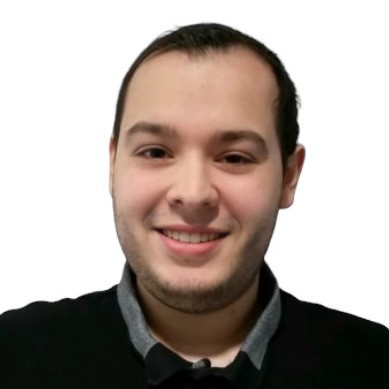
\includegraphics[width=.8in]{montoison.jpeg}
    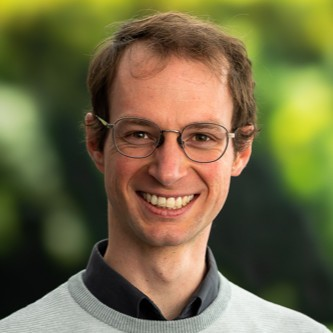
\includegraphics[width=.8in]{pacaud.jpeg}
    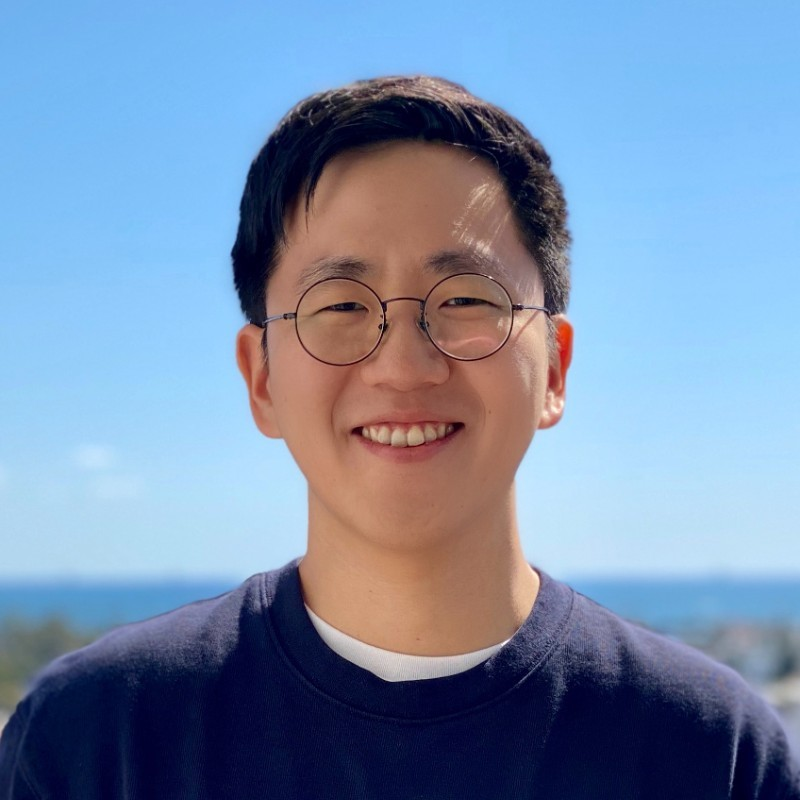
\includegraphics[width=.8in]{shin.jpeg}
    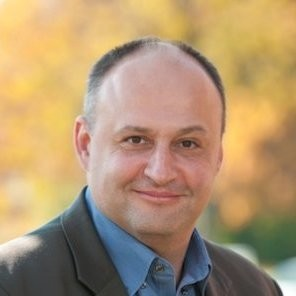
\includegraphics[width=.8in]{anitescu.jpeg}
  \end{center}
  \begin{itemize}
  \item Alexis Montoison @ Argonne National Lab
  \item François Pacaud @ MINES Paris-PSL (an ANL alumnus)
  \item Sungho Shin @ MIT (an ANL alumnus)
  \item Mihai Anitescu @ Argonne National Lab
  \item and friends... Michael Saunders, Dominic Orban, Armin Nurkanović, Anton Pozharskiy, Jean-Baptiste Caillau, ...
  \end{itemize}
\end{frame}

% ---------------------------
\section{Motivation}
% ---------------------------
\begin{frame}{GPU-based optimization}
  \begin{itemize}
  \item What is GPU? ---many-core accelerator with high memory bandwidth
  \item<2-> Traditionally used for graphics, now widely used for ML/AI workloads
  \item<3-> Classical optimization (mathematical programming; not ML training) has been considered \alert{unsuitable} for GPUs
  \item<4-> Many state-of-the-art solvers on CPUs rely on \alert{sparse direct factorizations}, which are viewed as \alert{difficult} to implement efficiently on GPUs
  \item<5-> This status quo is changing---the focus of this talk 
  \end{itemize}
\end{frame}

\begin{frame}{GPU-based optimization: current landscape}
  \begin{itemize}
  \item \alert{Factorization-free methods} have been the dominant approach:
    \begin{itemize}
    \item PDLP: first-order method for LPs \citep{applegatePracticalLargeScaleLinear2022,luCuPDLPFurtherEnhanced2025}
    \item {PCG} within ADMM for convex QPs \citep{schubigerGPUAccelerationADMM2020}
    \item ALM + IPM + PCG for nonlinear problems \citep{caoAugmentedLagrangianInteriorpoint2016}
    \end{itemize}
  \item<2-> These methods rely solely on \alert{GPU-friendly kernels}---\alert{\texttt{spmv}, \texttt{axpy}, \texttt{map}, \texttt{mapreduce}}---facilitating implementation on GPUs
  \item<3-> They scale to extremely large problems, but achieving high precision remains challenging
  \end{itemize}
  \visible<4->{
    \begin{center}
      \it Can we implement solvers based on \alert{second-order methods} and \alert{direct linear algebra} on GPUs?
    \end{center}
  }
  \refbr{
    \fullcite{applegatePracticalLargeScaleLinear2022}\\
    \fullcite{luCuPDLPFurtherEnhanced2025}\\
    \fullcite{schubigerGPUAccelerationADMM2020}\\
    \fullcite{caoAugmentedLagrangianInteriorpoint2016}
  }
\end{frame}

% ---------------------------
\section{Problem Setting: NLPs}
% ---------------------------
\begin{frame}{Our problem setting}{Large-scale, sparse, constrained nonlinear programs}
  \begin{itemize}
  \item \only<1>{
      We consider:
      \begin{align*}
        \min_{x^\flat\leq x \leq x^\sharp}&\; f(x) \\
        \text{s.t.}&\; g^\flat\leq g(x)\leq g^\sharp,
      \end{align*}
    }
    \only<2->{
      WLOG (via $a=b \iff a \geq b,\; b\geq a$), we consider:
      \begin{align*}
        \min_{x\in\mathbb{R}^n}&\; f(x) \\
        \text{s.t.}&\; g(x)\geq 0,
      \end{align*}
    }
    \visible<3->{... but will particularly focus on:}
    \begin{itemize}
    \item<3-> $f:\mathbb{R}^n\to\mathbb{R}$ and $g:\mathbb{R}^n\to\mathbb{R}^m$ twice continuously differentiable
    \item<4-> Generally \alert{nonconvex}---we only seek \alert{local solutions}
    \item<5-> $n$ and $m$ are large (millions or more)
    \item<6-> $\nabla g(x)$ and $\nabla^2_{xx} L(x,\lambda)$ are \alert{sparse} (tens of nonzeros per row)---$L(\cdot,\cdot)$ is the Lagrangian
    \end{itemize}
  \item<7-> Most existing solvers (e.g., Ipopt, KNITRO) are optimized for such problems
  \item<8-> Most important instances (e.g., energy systems, optimal control) fall into this category
  \end{itemize}
\end{frame}

% ---------------------------
\section{Software Structure}
% ---------------------------
\newcommand{\kktsystem}{%
  \begin{align*}
    \underbrace{
    \begin{bmatrix}
      \nabla^2_{x x} L(x,s,\lambda) + \delta_p I & & \nabla g(x)^\top
      \\ & S^{-1}\Lambda &  -I
      \\ \nabla g(x) & -I &  - \delta_d I
    \end{bmatrix}
    }_{\text{KKT matrix}}
    \underbrace{
    \begin{bmatrix}
      \phantom{-}d_x \\
      \phantom{-}d_s \\
      -d_\lambda
    \end{bmatrix}}_{\text{step direction}} =
    -\underbrace{\begin{bmatrix}
      \nabla f(x) - \nabla g(x)^\top \lambda\\
      \Lambda e - \mu S^{-1}e \\
      g(x) - s\\
    \end{bmatrix}}_{\text{residual to KKT conditions}},
  \end{align*}
}
\begin{frame}{NLP software stack---either on CPUs or GPUs}{{(1) algebraic modeling system}, {(2) NLP solver}, and {(3) sparse, direct linear solver}}
  \begin{itemize}
  \item<2-> \alert{Algebraic modeling systems} (e.g., JuMP, AMPL, CasADi) generate \alert{callback functions---$f(\cdot)$, $g(\cdot)$, $\nabla f(\cdot)$, $\nabla g(\cdot)$, $\nabla^2_{xx} L(\cdot,\cdot)$}---for \alert{NLP solvers}
  \item<3-> \alert{NLP solvers} (e.g., Ipopt, KNITRO) form \alert{KKT systems} to find step direction:
  \kktsystem
    where $s$ is slack; $S=\text{diag}(s)$; $\Lambda=\text{diag}(\lambda)$; and $\delta_p,\delta_d\geq 0$ are regularization parameters
  \item<4-> \alert{Sparse, direct linear solvers} (e.g., MA27, PARDISO) factorize and solve KKT systems; iterative method is typically not an option due to \alert{ill-conditioning}
  \end{itemize}
\end{frame}


\begin{frame}{Full NLP software stack on GPU---is it possible?}{{(1) algebraic modeling system}, {(2) NLP solver}, and {(3) sparse, direct linear solver}}
  \begin{itemize}
  \item Partially porting on GPU (e.g., AD or linear algebra only) is not sufficient---will be bottlenecked by CPU--GPU communication. We need \alert{all three components on GPU}
  \item<2-> Porting \alert{algebraic modeling system} is relatively straightforward. ExaModels.jl provides GPU-compatible modeling capabilities \citep{shinAcceleratingOptimalPower2024}---not the focus today
  \item<3-> Porting \alert{direct linear solver} is non-trivial; \alert{there is no drop-in replacement for MA27}
  \end{itemize}
  \medskip
  \visible<4->{
    \begin{block}{Our approach}
      {Adapt interior-point method (IPM) for NLPs} so that it can utilize {GPU direct linear solvers}
    \end{block}
  }
  \refbr{
    \fullcite{shinAcceleratingOptimalPower2024}
  }
\end{frame}
% ---------------------------
\section{Pivoting \& Inertia}
% ---------------------------

\begin{frame}{Linear algebra within IPM (on CPUs)}
  \begin{block}{Sparse LBL$^\top$ factorization \citep{duffMultifrontalSolutionIndefinite1983}}
    \vspace{-1em}
    \begin{align*}
      \begin{bmatrix}
        \nabla^2_{x x} L(x,s,\lambda) + {\color{magenta}\delta_p I} & & \nabla g(x)^\top
        \\ & S^{-1}\Lambda &  -I
        \\ \nabla g(x) & -I &  - {\color{magenta}\delta_d I}
      \end{bmatrix}
      =
      {\color{blue}P}\times {\color{red}Q}\times {\color{ForestGreen}L\times B\times L^\top}\times  {\color{red}Q}^\top\times  {\color{blue}P}^\top
    \end{align*}
  \end{block}
  \begin{itemize}
  \item<2-> ${\color{blue}P}$: Fill-in-reducing (and parallel-friendly) re-ordering (re-used across IPM iterations)
  \item<3-> ${\color{red}Q}$: Numerical pivoting (computed on-the-fly during factorization) \visible<7>{\textcolor{red}{$\longleftarrow$ main pain point}}
  \item<4-> ${\color{ForestGreen}LBL^\top}$: Factorization of permuted matrix (triangular, almost-diagonal)
  \item<5-> Additionally, pivots may be \alert{perturbed}, which must be corrected via \alert{iterative refinement}
  \item<6-> \alert{Factorization reveals inertia}---number of $+$, $0$, and $-$ eigenvalues; {primal-dual regularization {\color{magenta}$(\delta_p,\delta_d)$} is adjusted} to achieve correct inertia \citep{wachterImplementationInteriorpointFilter2006}
  \end{itemize}
  \refbr{
    \fullcite{duffMultifrontalSolutionIndefinite1983}\\ 
    \fullcite{wachterImplementationInteriorpointFilter2006}\\
    \fullcite{nocedalNumericalOptimization2006}
  }
\end{frame}

\begin{frame}{Pivoting-free IPM}{\cite{montoisonGPUImplementationSecondOrder2025}}
  \begin{itemize}
  \item Numerical pivoting is \alert{difficult} to implement on GPUs because it may \alert{incur irregular memory access} and \alert{destroy parallelism} \citep{swirydowiczLinearSolversPower2022}
  \item<2-> Existing GPU solvers (e.g., cuDSS) \alert{don't have adequately robust pivoting strategies}
  \item<3-> However, when pivoting is not required, \alert{GPU solvers (e.g., cuDSS) can be very efficient}
  \item<4-> Factorization may fail without \alert{numerical pivoting}, unless
    \begin{itemize}
    \item \alert{Symmetric quasi-definite} (SQD): factorization exists \citep{vanderbeiSymmetricQuasidefiniteMatrices1995} 
    \item \alert{Symmetric positive definite} (SPD): factorization exists and numerically stable
    \end{itemize}
  \end{itemize}
  \begin{center}
    \it
    \visible<5->{\alert{Can we make IPM pivoting-free?}}\\
    \visible<6->{(For now) can we reformulate KKT systems to be SPD or SQD?}
  \end{center}
  \refbr{
    \fullcite{montoisonGPUImplementationSecondOrder2025}\\
    \fullcite{vanderbeiSymmetricQuasidefiniteMatrices1995}\\
    \fullcite{swirydowiczLinearSolversPower2022}
  }
\end{frame}

% ---------------------------
\section{Option 1: Lifted KKT}
% ---------------------------
\begin{frame}{Option 0 (?): Vanila IPM + cuDSS}
  \begin{itemize}
  \item With MadNLP v0.8.12 + cuDSS v0.7.1, convergence is typically OK with small problems ($<10k$ variables), but \alert{fails frequently with larger problems} ($>10k$ variables)
  \item<2-> Linear solver relies on \alert{pivot perturbation} $\Rightarrow$ poor factorization accuracy $\Rightarrow$ iterative refinement failure $\Rightarrow$ \alert{forced primal-dual regularization} $\Rightarrow$ \alert{slow convergence or failure}
  \end{itemize}
  \medskip
  \begin{center}
    \visible<3>{
      As of now, using GPU direct solver with vanila IPM solver is \alert{not a viable option}
      }
  \end{center}
\end{frame}

\begin{frame}{Option 1: Lifted KKT method}{\cite{shinAcceleratingOptimalPower2024}}
\begin{itemize}
\item First, \alert{lift and relax equalities with small enough $\tau$} (the same as solver tolerances):
  \begin{align*}
    h(x)=0\quad \Longrightarrow \quad h(x) + s = 0 \quad\text{ and }\quad -\tau \leq s \leq\tau
  \end{align*}
\item<2-> \alert{Condense} the KKT system by eliminating slack/dual variables:
  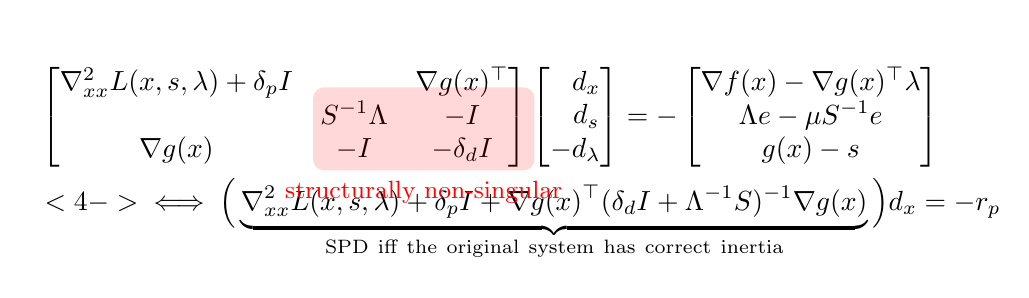
\begin{tikzpicture}
    \node[text width=\textwidth] at (0,0) {
      \begin{align*}
        &\begin{bmatrix}
          \nabla^2_{x x} L(x,s,\lambda) + \delta_p I & & \nabla g(x)^\top
          \\ & S^{-1}\Lambda &  -I
          \\ \nabla g(x) & -I &  - \delta_d I
        \end{bmatrix}
          \begin{bmatrix}
            \phantom{-}d_x \\
            \phantom{-}d_s \\
            -d_\lambda
          \end{bmatrix}
          =      
          -\begin{bmatrix}
            \nabla f(x) - \nabla g(x)^\top \lambda\\
            \Lambda e - \mu S^{-1}e \\
            g(x) - s\\
          \end{bmatrix}
        \\
        &
          \visible<4->{
          \iff
          \Big(\underbrace{\nabla^2_{xx} L(x,s,\lambda) + \delta_p I + \nabla g(x)^\top (\delta_d I + \Lambda^{-1} S)^{-1} \nabla g(x) }_{\text{\alert{SPD iff the original system has correct inertia}}}\Big) d_x = - r_p
          }
      \end{align*}
    };
    \visible<3>{
      \node[rounded corners,minimum width=80,minimum height=30,red,fill,opacity=.15] (shade) at (-1.15,.25) {};
      \node[align=center,anchor=north,font=\small,red] at (shade.south) {structurally non-singular}; 
    }
  \end{tikzpicture}
\item<5-> Enables numerically stable factorization \alert{without pivoting or excessive regularization}
\end{itemize}
\refbr{
  \fullcite{shinAcceleratingOptimalPower2024}
}
\end{frame} 

\begin{frame}{Option 1: Lifted KKT method---numerical results (AC OPF)}{\cite{montoisonGPUImplementationSecondOrder2025}}
  \begin{center}
    \scriptsize
    \begin{tabular}{|c|c|cc|cc|cc|cc|}
      \hline
      \multirow{ 3}{*}{\bfseries Tol} & \multirow{ 3}{*}{\bfseries Solver} & \multicolumn{2}{c|}{\textbf{Small}}& \multicolumn{2}{c|}{\textbf{Medium}}& \multicolumn{2}{c|}{\textbf{Large}}& \multicolumn{2}{c|}{\multirow{2}{*}{\textbf{Total}}}\\
      && \multicolumn{2}{c|}{nnz $<2^{18}$}& \multicolumn{2}{c|}{$2^{18}\leq$ nnz $<2^{20}$}& \multicolumn{2}{c|}{$2^{20}\leq$ nnz}&&\\
      &&  Solved & Time &  Solved & Time &  Solved & Time &  Solved & Time \\
      \hline\hline
      \multirow{2}{*}{$10^{-4}$} & MadNLP (GPU) & \textbf{31} & 0.4166 & \textbf{24} & \textbf{2.6380} & \textbf{11} & \textbf{3.7040} & \textbf{66} & \textbf{1.6979}  \\
      & Ipopt (CPU)& \textbf{31} & 0.3970 & \textbf{24} & 5.0697 & 11 & 38.5053 & \textbf{66} & 5.3817  \\
      \hline
      \multirow{2}{*}{$10^{-8}$} & MadNLP (GPU) & 30 & 2.5037 & \textbf{24} & \textbf{4.6016} & 10 & \textbf{12.8040} & 64 & \textbf{4.6228}  \\
      & Ipopt (CPU) & \textbf{31} & 0.5100 & \textbf{24} & 5.4292 & 11 & 37.7818 & \textbf{66} & 5.5541  \\
      \hline
    \end{tabular} 
  \end{center}
  \begin{itemize}\small
  \item \alert{Benchmark set}: AC optimal power flow \citep{babaeinejadsarookolaeePowerGridLibrary2021}
  \item \alert{Hardware}: NVIDIA GV100 GPU / Intel Xeon Gold 6130 CPU
  \item \alert{Time}: reported as SGM10$:= \prod_{i=1}^n (t_i + 10))^{1/n} - 10$ with max wall time 900s 
  \end{itemize}
  \visible<2->{
    \begin{block}{Observation}
      GPU solver is most effective for large instances solved up to moderate accuracy ($10^{-4}$)
    \end{block}
  }
  \refbr{
    \fullcite{montoisonGPUImplementationSecondOrder2025}\\
    \fullcite{babaeinejadsarookolaeePowerGridLibrary2021}
  }
\end{frame}

\begin{frame}{Option 1: Lifted KKT---numerical results (COPS)}{\cite{montoisonGPUImplementationSecondOrder2025}}
  \begin{center}
    \scriptsize
    \begin{tabular}{|c|c|cc|cc|cc|cc|}
      \hline
      \multirow{ 3}{*}{\bfseries Tol} & \multirow{ 3}{*}{\bfseries Solver} & \multicolumn{2}{c|}{\textbf{Small}}& \multicolumn{2}{c|}{\textbf{Medium}}& \multicolumn{2}{c|}{\textbf{Large}}& \multicolumn{2}{c|}{\multirow{2}{*}{\textbf{Total}}}\\
      && \multicolumn{2}{c|}{nnz $<2^{18}$}& \multicolumn{2}{c|}{$2^{18}\leq$ nnz $<2^{20}$}& \multicolumn{2}{c|}{$2^{20}\leq$ nnz}&&\\
      &&  Solved & Time &  Solved & Time &  Solved & Time &  Solved & Time \\
      \hline\hline
      \multirow{2}{*}{$10^{-4}$} & MadNLP (GPU) & \textbf{13} & \textbf{0.8665} & \textbf{15} & \textbf{4.8665} & \textbf{16} & \textbf{3.8194} & \textbf{44} & \textbf{3.2314}  \\
      & Ipopt (CPU) & \textbf{13} & 5.2315 & \textbf{15} & 15.9701 & 15 & 45.8411 & 43 & 19.2243  \\
      \hline
      \multirow{2}{*}{$10^{-8}$} & MadNLP (GPU) & \textbf{13} & \textbf{0.8575} & \textbf{16} & \textbf{1.5572} & \textbf{16} & \textbf{8.3549} & \textbf{45} & \textbf{3.3797}  \\
      & Ipopt (CPU) & \textbf{13} & 5.9413 & \textbf{15} & 17.6758 & 15 & 40.8639 & 43 & 19.2999  \\ 
      \hline
    \end{tabular}
  \end{center}
  \begin{itemize}\small
  \item \alert{Benchmark set}: COPS Benchmark \citep{dolanBenchmarkingOptimizationSoftware2001}
  \item \alert{Hardware}: NVIDIA GV100 GPU / Intel Xeon Gold 6130 CPU
  \item \alert{Time}: reported as SGM10$:= \prod_{i=1}^n (t_i + 10))^{1/n} - 10$, max wall time 900s
  \end{itemize}
  \visible<2>{
    \begin{block}{Observation}
      GPU solver is most effective for large instances solved up to moderate accuracy ($10^{-4}$)
    \end{block}
  }
  \refbr{
    \fullcite{montoisonGPUImplementationSecondOrder2025}\\
    \fullcite{babaeinejadsarookolaeePowerGridLibrary2021}
  }
\end{frame}

% ---------------------------
\section{Option 2: Hybrid KKT}
% ---------------------------
\begin{frame}{Option 2: Hybrid KKT system}{ \cite{golubSolvingBlockStructuredIndefinite2003,regevHyKKTHybridDirectiterative2023,pacaudCondensedspaceMethodsNonlinear2024}}
  \begin{itemize}
  \item We keep the equality constraints $h(x)= 0$ and eliminate the inequalities (slack/dual):
    \begin{align*}
      &\begin{bmatrix}
        K_{\text{cond}} + \delta_p I & \nabla h(x)^\top
        \\ \nabla h(x) &  - \delta_d I
      \end{bmatrix}
        \begin{bmatrix}
          \phantom{-}d_x \\
          -d_{\lambda}
        \end{bmatrix}
        =      
        -\begin{bmatrix}
          r_x\\
          r_{\lambda}
        \end{bmatrix}\\
      &\xRightarrow[\text{\tiny (w/o changing solution)}]{\text{\tiny Regularization}}
        \begin{bmatrix}
          K_{\text{cond}} + \delta_p I + \rho  \nabla h(x)^\top \nabla h(x)& \nabla h(x)^\top
        \\ \nabla h(x) &  - \delta_d I
      \end{bmatrix}
        \begin{bmatrix}
          \phantom{-}d_x \\
          -d_{\lambda}
        \end{bmatrix}
        =      
        -\begin{bmatrix}
          r_x'\\
          r_{\lambda}
        \end{bmatrix}
    \end{align*}
  \item<2-> Then, the Schur complement can be solved with an iterative method (e.g., CG)
    \begin{align*}
      \Bigg(\underbrace{\nabla h(x)^\top \Big(\overbrace{K_{\text{cond}} + \delta_p I + \rho  \nabla h(x)^\top \nabla h(x)}^{\tikz[overlay]{\node {\scriptsize \alert{SPD for sufficiently large $\rho$ iff correct inertia}};}} \Big)^{-1} \nabla h(x)}_{\text{converges to } I \text{ as } \rho\rightarrow \infty}  + \delta_d I \Bigg) d_{\lambda} = r'_{\lambda} 
    \end{align*}
  \end{itemize}
  \refbr{
    \fullcite{golubSolvingBlockStructuredIndefinite2003}\\
    \fullcite{regevHyKKTHybridDirectiterative2023}\\
    \fullcite{pacaudCondensedspaceMethodsNonlinear2024}
  }
\end{frame}

% ---------------------------
\section{Beyond IPM KKT}
% ---------------------------
\begin{frame}{Options 3, 4, 5, ...}
  \begin{itemize}
  \item There can be lots of other ways to implement pivoting-free solvers
  \item<2-> \alert{MadIPM}: Solver for convex quadratic programs; uses regularization to avoid pivoting \citep{montoisonGPUImplementationSecondOrder2025}
  \item<3-> \alert{MadNCL}: ALM-based algorithm---ALM is more \alert{GPU-friendly} due to the quadratic penalty term. Uses nonlinearly-constrained Lagrangian (NCL) formulation and applies condensation techniques \citep{montoisonMadNCLGPUImplementation2025}
  \item<4-> Directly solving augmented systems without pivoting? ---currently under investigation
  \end{itemize}
  \refbr{
    \fullcite{montoisonGPUImplementationSecondOrder2025}\\
    \fullcite{montoisonMadNCLGPUImplementation2025}
  }
\end{frame}

% ---------------------------
\section{Conclusion}
% ---------------------------
\begin{frame}{Concluding remarks}
  \begin{columns}
    \begin{column}{.5\textwidth}
      \begin{center}
        Check out our project page!\\
        \url{https://madsuite.org/}
      \end{center}
    \end{column}
    \begin{column}{.5\textwidth}
      \begin{center}
        This slide deck:\\
        \url{https://tinyurl.com/5n7nryx5}
      \end{center}
    \end{column}
  \end{columns}
  \vspace{2em}
  \begin{itemize}
  % \item It is an exciting time to develop optimization solvers!
  % \item<2-> With \alert{GPU direct solvers}, \alert{second-order methods} on GPUs has now become possible
  % \item<3-> To harness these GPU direct solvers, we need \alert{pivoting-free algorithms}
  \item Existing GPU solvers have focused on \alert{factorization-free} (e.g. first-order) methods, but
      \begin{align*}
        \text{GPU optimization solvers}
        &\supsetneq \text{Factorization-free solvers}\\
        &\visible<2->{\supset\text{Factorization-baesd, but \alert{pivoting-free} solvers}}
      \end{align*}
    \item<3-> We presented \alert{Lifted KKT} and \alert{Hybrid KKT}, but there can be many others
  \end{itemize}
\end{frame}

\AtNextBibliography{\tiny}
\setbeamertemplate{bibliography item}{}
\begin{frame}{References}
  \tikz[text width=1.1\textwidth,xscale=.9,transform shape]{
    \node at (current page.center) {\printbibliography[heading=none]};
  }
\end{frame}


\begin{frame}{}
  \joint{
    Joint work with:
    Alexis Montoison (Argonne),
    François Pacaud (MINES-Paris),
    Mihai Anitescu (Argonne)
  }
  \thispagestyle{empty}
  \titlepage
\end{frame}


\end{document}

%%% Local Variables:
%%% mode: LaTeX
%%% TeX-master: t
%%% TeX-master: t
%%% TeX-master: t
%%% End:


